\Appendix{}

\label{appendix:A}

\section{Polarizability}

The presence of an external electric field causes the electron distribution of a molecule (or an atom) to rearrange from its ground state configuration and the molecular geometry to distort. A typical source of an electric field is light (i.e., electromagnetic radiation), and a common situation for the above process is light-matter interaction. The change of the electronic structure results in an induced dipole moment within the molecule. The quantum mechanical description of this process involves the addition of the electric field interaction to the molecular Hamiltonian and the resulting Schrödinger equation is commonly solved employing a perturbation approach. The response of the electronic structure following the perturbation of the original Hamiltonian can be considered using response theory.
If the applied electric field is weak, the induced dipole moment ($\mu_I$) varies linearly with the applied electric field strength ($\varepsilon$) and the constant of proportionality is the polarizability ($\alpha$). As the electric field strength increases, higher order terms in the field strength have to be included in the description of the induced dipole moment as shown in eqn (1). The total dipole moment ($\mu$) is the sum of permanent ($\mu_0$) and induced ($\mu_I$) dipole moment. The coefficients of the higher order terms are the hyperpolarizabilities of different order ($\beta$,$\gamma$,…). The latter are the source of important non-linear optical (NLO) effects. 

\begin{align}
 \mu = \mu_0 +  \alpha  \varepsilon + \frac{1}{2}  \beta  \varepsilon ^{2} +\frac{1}{6}   \gamma   \varepsilon ^{3}+...
\end{align}
 

The relationship between the polarizability and energy of a molecular system can be obtained \via\ a Taylor expansion of the energy in the electric field strength as shown in eqn (2). The derivative of the energy with respect to the electric field is simply the negative of the dipole moment as shown in the equation (3). Comparing eqns (1) and (3), we can readily obtain the expressions for permanent dipole moment, polarizability, and hyperpolarizabilities as shown in eqn (4). These expressions give the link between the properties we are interested in and the energy, which can be calculated using the perturbation theory. 

\begin{align}
 E =E(0) +    \bigg( \frac{dE}{d \varepsilon } \bigg) \varepsilon  + \frac{1}{2!}   \bigg( \frac{ d^{2} E}{d  \varepsilon^{2}  }\bigg) \varepsilon^{2}+\frac{1}{3!}   \bigg( \frac{ d^{3} E}{d  \varepsilon^{3}  }\bigg) \varepsilon^{3}+...
\end{align}

\begin{align}
 \mu  =-\bigg( \frac{dE}{d \varepsilon } \bigg) \varepsilon  - \bigg( \frac{ d^{2} E}{d  \varepsilon^{2}  }\bigg) \varepsilon-\frac{1}{2}   \bigg( \frac{ d^{3} E}{d  \varepsilon^{3}  }\bigg) \varepsilon^{2}- ...
\end{align}

\begin{align}
 \mu_0  =-\bigg( \frac{dE}{d \varepsilon } \bigg) , \; \alpha =- \bigg( \frac{ d^{2} E}{d  \varepsilon^{2}  }\bigg), \; \beta= -  \bigg( \frac{ d^{3} E}{d  \varepsilon^{3}  }\bigg), \; \gamma = - \bigg( \frac{ d^{4} E}{d  \varepsilon^{4}  }\bigg) 
\end{align}


\subsection{Static Polarizability}

The time-independent perturbation expression for the energy is given in eqn (5). The zeroth-order Hamiltonian is the original molecular Hamiltonian, the first-order Hamiltonian is the dipole moment operator $\varepsilon$$\mu$, and higher-order Hamiltonians do not have to be considered in this problem, so that the energy can be rewritten as eqn (6). Using this expression and eqn (4), the polarizability can be written as eqn (7). Using this expression, the mean (isotropic) electric polarizability can be written as eqn (8).
   
\begin{align}
 E =E_0^{(0)} + \expval{H^{(1) }}{0} +
 \sum_n  \frac{\mel{0}{H^{(1)}}{n}\mel{n}{H^{(1)}}{0}}{ \Delta E_{n0} }+ ...
\end{align}

\begin{align}
E =E_0^{(0)} - \expval{\mu}{0}\varepsilon +
\sum_n  \frac{\mel{0}{\mu}{n}\mel{n}{\mu}{0}}{ \Delta E_{n0} } \varepsilon^2+ ...
\end{align}

\begin{align}
\alpha =-2\sum_n  \frac{\mel{0}{\mu}{n}\mel{n}{\mu}{0}}{ \Delta E_{n0} }
\end{align}

\begin{align}
\alpha =\frac{1}{3}\big(\alpha_{xx}+\alpha_{yy}+\alpha_{zz}\big)=\frac{2}{3}\sum_n  \frac{\abs{\mu_{n0}}^2}{ \Delta E_{n0} }
\end{align}

The SI unit of polarizability is C$^2$m$^2$J$^{-1}$. The polarizability volume ($\alpha$') is also sometimes used instead of the polarizability as this can be a more convenient way to represent the polarizability (eqn (9)). The polarizability volume is expressed generally in \AA$^3$.

\begin{align}
\alpha' =\frac{\alpha}{4\pi\epsilon_0}
\end{align}


\subsection{Dynamic Polarizability} 

The eqn (5), which is the time-independent perturbation expression for energy, cannot be used to determine the dynamic polarizability. Thus, in order to determine the dynamic polarizability, $\alpha$($\omega$), we need to solve the time-dependent perturbation theory. Using the time-dependent wavefunction, the mean dynamic polarizability as shown in eqn (10) can be determined. It should be noted that as $\omega\rightarrow $0, the expression will be reduced to a static polarizability equation. It can also be noted that as $\omega\rightarrow \infty$, the polarizability goes to zero which is because the field changes so rapidly for the electrons to respond to the changing field. The electrons cannot contribute to the induced dipole moment if the applied field is changing very fast. 

\begin{align}
\alpha(\omega) =\frac{1}{3}\big(\alpha_{xx}+\alpha_{yy}+\alpha_{zz}\big) =\frac{2}{3\hbar}\sum_n  \frac{\omega_{n0}\abs{\mu_{n0}}^2}{ {\omega_{n0}}^2 - \omega^2}
\end{align}

\subsection{Relative Permittivity and the Electric Susceptibility}

The electric susceptibility ($\chi_e$) of a medium is defined in eqn (11), where P is the polarization and $\epsilon_0$ is the vacuum permittivity. In presence of an external electric field, a molecule experiences a local field ($\varepsilon^*$), rather than the applied one. The local electric field is the combination of external field and the field resulting from the electric dipoles present in the system. The local electric field is related to polarization as shown in eqn (12), where $N$ is the number density of molecules. 

\begin{align}
\chi_e=\frac{P}{\epsilon_0 \varepsilon}
\end{align}

\begin{align}
\varepsilon^*=\frac{P}{\alpha N}
\end{align}

The relationship between the local electric field and the applied electric field is given in the eqn (13), which assumes that the medium is a continuous dielectric. This is called as Lorentz local field expression. Using the eqn (12) and eqn (13), the polarization can be expressed as eqn (14). Comparing this expression with the eqn (11), the susceptibility can be written as eqn (15). The relative permittivity ($\epsilon_r$) of the medium is related to the susceptibility as shown in the eqn (16). Thus, the relation between the permittivity and polarizability can be determined as shown as eqn (17). 


\begin{align}
\varepsilon^* = \varepsilon + \frac{P}{3\epsilon_0}
\end{align}

\begin{align}
P = \bigg(\frac{3\alpha N}{3\epsilon_0 - \alpha N}\bigg)\epsilon_0 \varepsilon
\end{align}

\begin{align}
\chi_e = \bigg(\frac{\alpha N/\epsilon_0}{1 - \alpha N/3\epsilon_0}\bigg)\epsilon_0 \varepsilon
\end{align}

\begin{align}
\epsilon_r = \chi_e + 1
\end{align}

\begin{align}
\epsilon_r = \frac{1 + 2\alpha N / 3 \epsilon_0}{1 - \alpha N / 3 \epsilon_0}
\end{align}


\subsection{Refractive Index}

Refractive index (RI; $n_r$) can be related to $\epsilon_r$ using the Maxwell’s equations. The Maxwell’s equations are shown in the eqn (18), where $E$ is the electric field strength, ρ is the charge density, $D$ is the electric displacement, $H$ is the magnetic field strength and $B$ is the magnetic induction. The units for these equations are given in SI units. The relations between these fields can written as shown in eqn (19), where $\epsilon_r$ is the electric permittivity and $\mu_r$ is the magnetic permeability. 

\begin{align}
\nabla D = \rho,\; \nabla B = 0,\; \nabla \times E = - \frac{\partial B}{\partial t},\; 
\nabla \times H = \frac{\partial D}{\partial t}
\end{align}

\begin{align}
D = \epsilon_r \epsilon_0 E,\; B = \mu_r \mu_0 H
\end{align}

The propagation of light through any medium can be determined by the wave equation, which can be derived by considering the eqn (20). The left hand side of this eqn can be simplified as shown in eqn (21), whereas the right hand side can be simplified as shown in eqn (22). Comparing these simplified eqns yields the eqn (23). Thus, the velocity of light in the medium can be written as shown in the eqn (24). 

\begin{align}
\nabla \times (\Delta \times E) = - \nabla \times \bigg(\frac{\partial B}{\partial t}\bigg)
\end{align}

\begin{align}
\nabla \times (\nabla \times E) = \nabla \times (\nabla E) -(\Delta^2E) = - \nabla^2E \end{align}

\begin{align}
\nabla \times \big(\frac{\partial B}{\partial t}\big) = 
\frac{\partial}{\partial t}(\nabla \times \mu_r \mu_0 H)= \mu_r \mu_0 \frac{\partial^2}{\partial t^2}D = \mu_r \mu_0 \epsilon_r \epsilon_0 \frac{\partial^2}{\partial t^2}E
\end{align}

\begin{align}
\nabla^2 E = \mu_r \mu_0 \epsilon_r \epsilon_0 \frac{\partial^2}{\partial t^2}E
\end{align}

\begin{align}
C = \frac{1}{\sqrt{\mu_r \mu_0 \epsilon_r \epsilon_0 }}
\end{align}

As the refractive index is defined as the ratio between velocity of light in vacuum ($C_o$) and the velocity of light in the medium ($C$), the refractive index can be written as eqn (25). Assuming that the material is non-magnetic ($\mu_r=1$), it follows that the refractive index is the square root of the relative permittivity of the medium. Thus, using the eqn (17), the refractive index of a medium can be written as eqn (26). If the refractive index does not differ much from 1, the refractive index can be represented as eqn (27).

\begin{align}
n_r = \frac{C_0}{C} = \sqrt{\mu_r\epsilon_r}
\end{align}

\begin{align}
n_r = {\bigg(\frac{1 + 2\alpha N / 3 \epsilon_0}{1 - \alpha N / 3 \epsilon_0}\bigg)}^{1/2}
\end{align}

\begin{align}
n_r \approx 1 + \frac{\alpha N}{2 \epsilon_0}
\end{align}

Because refractive index of material is a property dependent on the frequency of the oscillating electric field, we have to use the dynamic polarizability, $\alpha$($\omega$), of the molecule. Thus, using the eqn (10) for the dynamic polarizability and eqn (27), the refractive index can be determined as a function of the frequency as


The dependence of refractive index with the frequency can be seen in the Fig.\ \ref{fig:RI_freq}. It can be seen that as the frequency goes to zero, i.e. at infinite wavelength, the refractive index becomes a constant value. A singularity can be observed at the resonance ($\omega = \omega_{n0}$), this is because the perturbation theory breaks down close to this point. At higher frequencies ($\omega>\omega_{n0}$), the refractive index is shown to have a value less than 1. In my project, I will be calculating the refractive index at infinite wavelength which can be determined using the mean static polarizability values. This is because it is relatively easy to calculate the refractive index this way. Further, it has been shown that the values of the RI obtained through this way is in good agreement with the experimental values. More details are provided in the next section of this appendix. 


\begin{figure}[htbp] 
	\centering
	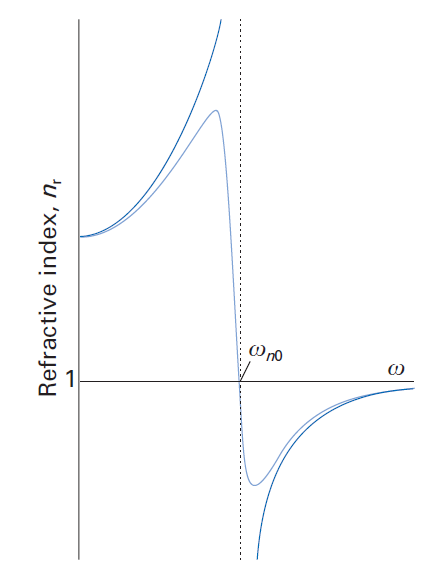
\includegraphics[width=0.4\textwidth]{Appendix-A/Figures/RI_vs_omega.png}
	\caption{Dispersion characteristic of the refractive index: Excited states are marked by singularities, and in the frequency range below, the RI values converges asymptotically towards the constant value \cite{Atkins2011}.} 
	\label{fig:RI_freq} 
\end{figure}  


\section{Modeling of the Refractive Index of Polymers}

As explained in the previous section, the RI value of a material is connected to the electric polarizability and can thus be obtained from quantum chemical linear response calculations. An array of electronic structure methods has been used to determine the RI of various materials \cite{Ando2006, Rocquefelte2004, Jensen1983, Rabah2003, Amrani2006, Reshak2014, Azam2013,Baev2007,Asai2011,Takano2010,Seto2010}, including organic polymers \cite{Ksianzou2006, Zeinalipour-Yazdi2008, Yu2007,Holder2006,Ortyl2003,}. %A selection of representative studies have been listed in Table 1, and the different modeling approaches have been highlighted.

It is fairly easy to calculate the RI value given the dynamic molecular polarizability (and the number density) of a material using the Lorentz-Lorentz equation. However, it is generally quite challenging to determine the necessary dynamic polarizability, as it formally involves solving the time-dependent Schr\"odinger equation and/or scanning through the range of relevant frequencies. Consequently, relatively few studies have considered the polarizability dispersion of organic polymers \cite{Rowan2011, Lenz2011}. 

Although the RI value is a frequency-dependent property, its variation in the visible region is in fact often relatively small. This assumes the absence of low-lying excited states, which would render a material unsuitable for optical applications in the first place. Large variations can be observed in the ultraviolet region where resonances with the excited state manifold become the dominant feature, however, stability considerations would prohibit organic polymers to be used for high-energy applications anyways. Towards the infrared the RI decreases monotonically and becomes constant. Fig.\ \ref{fig:exp_RI_wl}, shows the experimental results for diamondoid containing polymers, which exemplify this behavior. Fig.\ \ref{fig:calc_RI_wl} shows the quantum chemical result for amber, which exhibits the same trend: We see significant dispersion in the region below 250 nm where the material starts to absorb the incident radiation and becomes electronically excited. Beyond 250 nm, the RI value tapers off and becomes essentially constant throughout the visible and infrared range. The asymptotic RI value corresponds to the one that can be derived from the static polarizability. The latter can be computed much more easily than the frequency-dependent value. It only requires a single linear response calculation without explicit time dependence, and is thus much less demanding in terms of computer-time and numerical stability. We can conclude that the RI values obtained from static polarizability calculations form a close lower bound for the frequency dependent values in the relevant spectral range. This approach has been used extensively in the past and has given very good agreement with the experimental results \cite{Ksianzou2006, Zeinalipour-Yazdi2008, Lee2011, Park2011, Isborn2007, Azim-Araghi2012}. 

The RI values based on static polarizability calculations are thus a useful indicator to the overall performance of a candidate compound, in particular for the purpose of a large-scale screening of potential candidates. A more detailed analysis of the dispersion characteristic and of other relevant properties (such as the stability, low-energy excitations, permittivity, color, etc) are obviously necessary to come to a full assessment regarding the prospects of a candidate compound. We will attempt to develop heuristic correction and calibration schemes to account for some of these effects. 

\begin{figure}[htbp] 
	\centering
	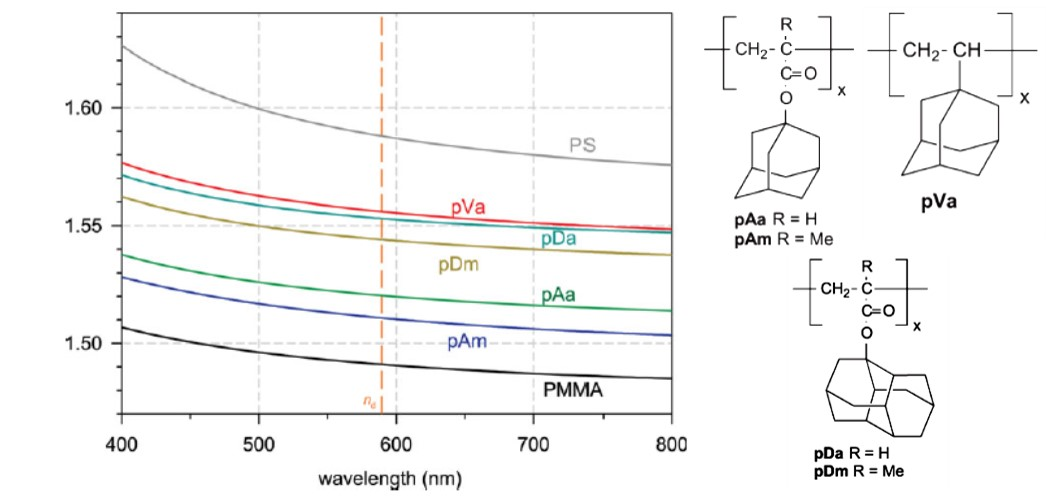
\includegraphics[width=0.9\textwidth]{Appendix-A/Figures/exp_RI_wl.jpg}
	\caption{Experimental dispersion of the RI values for a set of organic polymers \cite{Robello2013}.} 
	\label{fig:exp_RI_wl} 
\end{figure}  

\begin{figure}[htbp] 
	\centering
	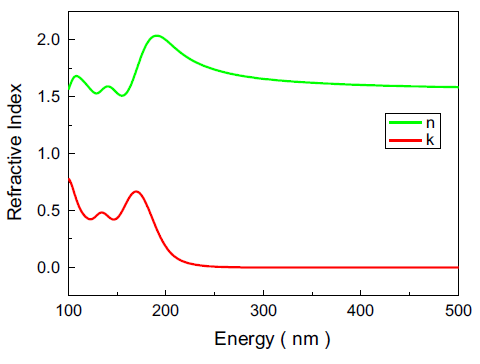
\includegraphics[width=0.6\textwidth]{Appendix-A/Figures/calc_RI_wl.png}
	\caption{Wavelength-dependent RI values determined by quantum chemical modeling \cite{Rao2013}. (Note: the imaginary component shown in red will not be included in the present discussion as it goes beyond the scope of our current work).} 
	\label{fig:calc_RI_wl} 
\end{figure}  
